\documentclass[xcolor=table,aspectratio=169,dvipsnames,english]{beamer}
\usepackage{bm}
\usepackage[utf8]{inputenc}
\usepackage{color}

\usepackage[british]{babel} % decent hyphenation, avoiding e.g. anal-ysis
\usepackage[iso]{isodate}
\usepackage{sansmath}
\usepackage{booktabs}
\usepackage{graphicx}
\usepackage{graphviz}
\usepackage{makecell}
\usepackage{minted}
\usepackage{multicol}
\usepackage{siunitx}
\usepackage{subcaption}
\usepackage[section]{placeins}

% Needs to be loaded after hyperref
\usepackage{cleveref}

% PythonTeX
\usepackage[autoprint=false, gobble=auto, keeptemps=all, pyfuture=all]{pythontex} % create figures on-line directly from python!
\usepackage{pgf}
%\input{/usr/share/repsep/functions.py}
\input{functions.py}
\begin{pythontexcustomcode}[begin]{py}
pytex.add_dependencies(
	'lib/utils.py',
	'lib/categorical.py',
	'data/JogB.tsv'
	)
\end{pythontexcustomcode}
% Single-session PythonTeX codeblocks
\newcounter{pysessioncounter}
\newcommand{\sessionpy}{%
          \edef\sessionpysession{session\arabic{pysessioncounter}}%
            \stepcounter{pysessioncounter}%
              \expandafter\py\expandafter[\sessionpysession]}

% SIunitx customizations detect-all will use the current font for typesetting
\sisetup{per-mode=symbol, detect-all, range-units = single}
\newcommand\SIci[5]{\SI{#1}{#2}, {#3}CI: \SIrange{#4}{#5}{#2}}

% Fix for matplotlib PGF wonkiness which isn't interpreted correctly by pdflatex
\DeclareUnicodeCharacter{2212}{-}


%\hypersetup{
%    colorlinks=true,
%    urlcolor=cyan
%}

%BIBLIOGRAPHY
% see https://mirror.foobar.to/CTAN/macros/latex/contrib/biblatex/doc/biblatex.pdf for available styles
\usepackage[backend=bibtex,style=numeric,natbib=true]{biblatex}
\addbibresource{bib.bib}
\addbibresource{old_bib.bib}

% Article-specific configuration
\begin{pythontexcustomcode}[begin]{py}
DOC_STYLE="slides/main.conf"
pytex.add_dependencies(
	DOC_STYLE,
	'slides/1col.conf',
	)
\end{pythontexcustomcode}

% Custom beamer styling and colors
\setbeamersize{text margin left=0.8em,text margin right=0.8em}
\setbeamertemplate{bibliography item}{\insertbiblabel}

\usecolortheme[RGB={199,199,199}]{structure}
\usetheme{Dresden}

\captionsetup[figure]{labelformat=empty}

\definecolor{dy}{RGB}{202,202,0}
\definecolor{rsblue}{HTML}{00a3cc}
\definecolor{mg}{gray}{0.30}
\definecolor{lg}{gray}{0.60}
\definecolor{vlg}{gray}{0.78}
\definecolor{tlg}{gray}{0.88}

\setbeamercolor{caption name}{fg=lg}
\setbeamercolor{caption}{fg=lg}
\setbeamercolor{author}{fg=lg}
\setbeamercolor{institute}{fg=lg}
\setbeamercolor{date}{fg=lg}
\setbeamercolor{title}{fg=mg}
\setbeamertemplate{caption}{\centering\insertcaption\par}
\setbeamertemplate{navigation symbols}{}

% Navigation symbols are too far down by default
% To further adjust edit the pt numbers before and after `\insertnavigation`
\makeatletter
\defbeamertemplate*{headline}{my miniframes theme}
{%
        \begin{beamercolorbox}[colsep=1.5pt]{upper separation line head}
        \end{beamercolorbox}
        \begin{beamercolorbox}{section in head/foot}
                \vskip1pt\insertnavigation{\paperwidth}\vskip3pt
        \end{beamercolorbox}%
        \ifbeamer@theme@subsection%
                \begin{beamercolorbox}[colsep=1.5pt]{middle separation line head}
                \end{beamercolorbox}
                \begin{beamercolorbox}[ht=2.5ex,dp=1.125ex,%
                        leftskip=.3cm,rightskip=.3cm plus1fil]{subsection in head/foot}
                        \usebeamerfont{subsection in head/foot}\insertsubsectionhead
                \end{beamercolorbox}%
        \fi%
        \begin{beamercolorbox}[colsep=1.5pt]{lower separation line head}
        \end{beamercolorbox}
}
\makeatother


\title{Multimodal Generative Learning on the MIMIC-CXR Database}
\subtitle{A presentation of my semester project}
\author{Hendrik Klug}
\institute{Institute for Electrical Engineering, ETH}
\begin{document}
    \begin{frame}
        \titlepage
    \end{frame}


    \section{Introduction}

    \begin{frame}
        In this work, we applied a method for \textbf{self-supervised},\textbf{multimodal} and \textbf{generative} training from \cite{thomas_multimodal} on medical data from the MIMIC-CXR Database (\cite{johnson2019mimic}).
    \end{frame}

    \subsection{Multimodal, Unsupervised, Generative models}
    \begin{frame}{Self-supervised, multimodal, generative learning?}
        \py{pytex_printonly(script='scripts/generalidea_graph.py', data = '')}
    \end{frame}

    \begin{frame}{Multimodal, Unsupervised Generative Learning On Medical Data}
        \begin{itemize}
            \item No need for labeled data
        \end{itemize}
    \end{frame}
    
    \begin{frame}{No need for labeled data}
    Since the model is trained to only reconstruct the input images, it does not need labeled data for training.
    This is a big advantage over other methods because labeled data in the medical domain is rare and hard to acquire because it requires manual expert input.\\
    \\
    \pause
    However, since the data belonging to different classes will be represented in a different manner in the learned latent representation of the model, the model can still be used for data classification.
        
    \end{frame}
    
        \begin{frame}{}
        \begin{figure}
            \centering

            \begin{tikzpicture}[model/.style={rectangle, draw=red!60, fill=red!5, very thick, minimum height=20mm, minimum width=20mm},lr/.style={ellipse, draw=blue!60, fill=blue!5, very thick, minimum height=30mm,  minimum width=60mm},t/.style={ellipse, draw=green!60, fill=green!5, very thick, minimum size=5mm},front/.style={ellipse, draw=orange!60, fill=orange!5, very thick, minimum size=5mm},]
            	\node[t] (cl1) {class 1};
            	%\node[front, below of=cl1] (cl2) {class 1};
            	\node[model, right of=cl1, xshift=2cm, yshift=-0.5cm] (model) {Model};
            	\node[lr, right of=model, xshift=4cm] (lr) {};
            	\node[t, right of=lr, xshift=-1.8cm, yshift = -0.5cm] (cl1_) {class 1};
            		\node[right of=model, xshift=4cm, yshift=0.85cm] (lr_string) {\textbf{Latent Representation}};
            
            	%\node[front, right of=lr, xshift=0.9cm, yshift = 0.3cm] (cl2_) {class 2};
            	\draw[->,green!60] (cl1) -- (model);
            	%\draw[->,orange!60] (cl2) -- (model);
            	\draw[->,green!60] (model) -- (cl1_);
            	%\draw[->,orange!60] (model) -- (cl2_);
            \end{tikzpicture}
        \end{figure}

    \end{frame}
    
    
    \begin{frame}{}
            \begin{figure}
            \centering
        \begin{tikzpicture}[model/.style={rectangle, draw=red!60, fill=red!5, very thick, minimum height=20mm, minimum width=20mm},lr/.style={ellipse, draw=blue!60, fill=blue!5, very thick, minimum height=30mm,  minimum width=60mm},t/.style={ellipse, draw=green!60, fill=green!5, very thick, minimum size=5mm},front/.style={ellipse, draw=orange!60, fill=orange!5, very thick, minimum size=5mm},]
	\node[t] (cl1) {class 1};
	\node[front, below of=cl1] (cl2) {class 2};
	\node[model, right of=cl1, xshift=2cm, yshift=-0.5cm] (model) {Model};
	\node[lr, right of=model, xshift=4cm] (lr) {};
	\node[right of=model, xshift=4cm, yshift=0.85cm] (lr_string) {\textbf{Latent Representation}};
	\node[t, right of=lr, xshift=-1.8cm, yshift = -0.5cm] (cl1_) {class 1};
	\node[front, right of=lr, xshift=0.9cm, yshift = 0.3cm] (cl2_) {class 2};
	\draw[->,green!60] (cl1) -- (model);
	\draw[->,orange!60] (cl2) -- (model);
	\draw[->,green!60] (model) -- (cl1_);
	\draw[->,orange!60] (model) -- (cl2_);
\end{tikzpicture}
        \end{figure}

    \end{frame}
    

    
        \begin{frame}{Multimodal, Unsupervised Generative Learning On Medical Data}
        \begin{itemize}
            \item No need for labeled data
            \item Can extract features from multiple modalities that exist in the medical domain:
            \pause
                \begin{itemize}
                    \item Scans from multiple angles or scanning technologies
                    \item Text reports
                    \item Electronic health records
                \end{itemize}
            \pause
            \item Can generate \textit{coherent} samples from one input modality
        \end{itemize}
    \end{frame}
    
    \section{Background}

    \subsection{The MoPoE-VAE (\cite{thomas_gener-ELBO})}
    \begin{frame}{The Mixture-of-Products-of-Experts-VAE}
    \pause
        Combination of:
        \begin{itemize}
            \item The Product-of-Experts (PoE) from \cite{wu2018multimodal}
            \item The Mixture-of-Experts (MoE) from \cite{shi2019variational}
        \end{itemize}
        \vspace{\baselineskip}
        Both present a different choice for the joint posterior approximation function.
    \end{frame}
    
    \begin{frame}{The PoE-VAE}

        \begin{itemize}
            \item Uses a geometric mean: the joint posterior is a product of individual posteriors
            %p(z|x_1,...,x_N)) \propto p(z) \prod _{i=1} ^N \tilde{q}(z|x_i)
            \begin{equation}
                q_{\Phi}(z|x_{1:M})=\prod _m q_{\Phi_m}(z|x_m)
            \end{equation}
            \item Results in a good approximation of the joint distribution but struggles in optimizing the individual experts.
            \item If one of the expert is miscalibrated (bad initialisation, overconfidence), it will perturb the whole joint distribution. 
        \end{itemize}
    \end{frame}

    \begin{frame}{The MoE-VAE}
        \begin{itemize}
            \item Uses an arithmetic mean
            \begin{equation}
                q_{\Phi}(z|x_{1:M})=\sum _m \alpha_m\cdot q_{\Phi_m}(z|x_m)
            \end{equation}
            \item Optimizes individual experts well but is not able to learn a distribution that is sharper than any of its experts.
        \end{itemize}

    \end{frame}

    \begin{frame}{The Mixture-of-Products-of-Experts-VAE}
        The generalized multimodal ELBO utilizes the PoE to get the posterior approximation of a subset $\xsubset \in \mathcal{P}(\mathbb{X})$:

        \begin{equation}
            \tilde{q}_{\phi}(\textbf{z}|\xsubset)=PoE(\{q_{\phi_j}(\textbf{z}|\textbf{x}_j) \forall \textbf{x}_j \in \xsubset\}) \propto \prod _{\textbf{x}_j \in \xsubset}q_{\phi_j}(\textbf{z}|\textbf{x}_j)
        \end{equation}
        And the MoE to get the joint posterior:
        \begin{equation}
            q_{\phi}(\textbf{z}|\mathbb{X}) = \frac{1}{2^3} \sum _{\textbf{x}_k \in \mathbb{X}} \tilde{q}_{\phi} (\textbf{z}|\mathbb{X}_k)
        \end{equation}
    \end{frame}

    \begin{frame}{}

        \py{pytex_printonly(script='scripts/mopoe_graph.py', data = '')}

    \end{frame}


    \section{Methods}

    \subsection{The MIMIC-CXR Database}
    \begin{frame}{The dataset}
        The MIMIC-CXR Database \cite{johnson2019mimic} is a large publicly available dataset of chest radiographs with free-text radiology reports containing 377,110 images corresponding to 227,835 radiographic studies performed at the Beth Israel Deaconess Medical Center in Boston, MA.

    \end{frame}

    \begin{frame}
        \py{pytex_fig('scripts/rand_sample_from_dataset.py', conf='slides/dataset.conf', label='dataset_samples', caption='Samples from the dataset.')}
    \end{frame}

    \begin{frame}{The labels}
        Since the multiple labels from the dataset are highly imbalanced, we created a label "Finding", indicating if the sample is labeled with any pathology.\\
        There are \py{boilerplate.print_finding_counts()} samples that are annotated with the "Finding" label in the training set and \py{boilerplate.print_nofinding_counts()} samples that are not.
    \end{frame}

    \begin{frame}{The word encoding}
        Every word that occurs at least \py{boilerplate.print_flag_attribute('word_min_occ')} times in all the text reports is mapped to an index.\\
        Using this mapping each sentence is encoded into a sequence of indices.\\
        The output of the decoder is in a one-hot-encoded format.
        
        \pause
        \vspace{\baselineskip}

        \small{
        "Heart size is normal." $\rightarrow [0,1,2,3] \rightarrow$ Model $\rightarrow
        \begin{bsmallmatrix}
            1 & 0 & 0 & 0\\
            0 & 1 & 0 & 0\\
            0 & 0 & 1 & 0\\
            0 & 0 & 0 & 1\\
        \end{bsmallmatrix}$
        $\rightarrow [0,1,2,3] \rightarrow$ "Heart size is normal."}
    \end{frame}

    \subsection{The model architecture}
    \begin{frame}{The model}
        The MoPoE-VAE has an encoder and decoder for each modality, in this work we used a ResNet type architecture for all encoders and decoders.
    \end{frame}

    \begin{frame}{Resnet}
        Residual Neural Networks are a popular architecture for deep learning models.
        Since its publication in an article from \cite{he2016deep}, it has been widely used (cited over 70453 times) for image recognition tasks.
        \begin{figure}
            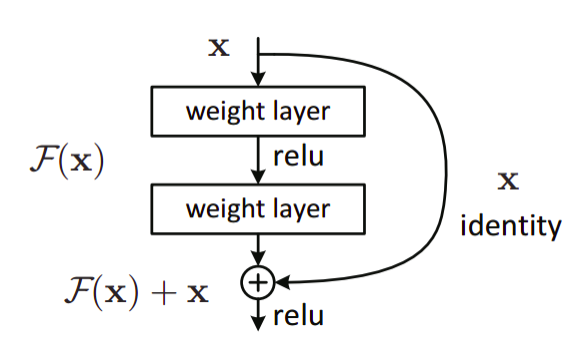
\includegraphics[width=0.3\textwidth, keepaspectratio]{slides/Residual_block}
            \caption{Residual learning: a building block. Taken from \cite{he2016deep}.}
        \end{figure}

    \end{frame}

    \subsection{Evaluation methods}
    
    \begin{frame}{Evaluation Methods}
        \begin{itemize}
            \item Evaluation of the separability of the latent representation
            \item Evaluation of the generation coherence
        \end{itemize}
    \end{frame}
    
    \begin{frame}{Evaluation of the latent representation}
        \begin{figure}[!h]
            \centering
            \begin{tikzpicture}

                \begin{scope}[blend group = soft light]
                    \fill[blue!40!white]   (0:0) ellipse (6cm and 3cm);
                    \fill[green!40!white] (0:-2) ellipse (1.5cm and 2cm);
                    \fill[red!40!white]  (0:2) ellipse (1.5cm and 2cm);
                    \draw [-,ultra thick] (0,-1.5) -- (0,1.5);
                \end{scope}
                \node at (0:-2)   {"No Finding"};
                \node at (0:2)   {"Finding"};
                \node at (90:2.3) [font=\Large] {Latent Representation};
            \end{tikzpicture}
        \end{figure}

    \end{frame}
    
    \begin{frame}{Evaluation of the latent representation}
        \begin{figure}[!h]
            \centering
            \begin{tikzpicture}

                \begin{scope}[blend group = soft light]
                    \fill[blue!40!white]   (0:0) ellipse (6cm and 3cm);
                    \fill[green!40!white] (0:-1) ellipse (3cm and 2cm);
                    \fill[red!40!white]  (0:1) ellipse (3cm and 2cm);
                \end{scope}
                \node at (0:-2)   {"No Finding"};
                \node at (0:2)   {"Finding"};
                \node at (90:2.3) [font=\Large] {Latent Representation};
            \end{tikzpicture}
        \end{figure}    
    \end{frame}

    \begin{frame}{Evaluation of the generation coherence}
        To evaluate the coherence of the generated samples, they are classified using trained ResNet classifiers.
        If all modalities of a sample, generated and given as conditioner, are classified as having the same label, they are considered coherent.
    \end{frame}

    \begin{frame}{Hyper-parameter Selection}
        We used a simple grid search to find the best hyperparameters, retaining the parameter values that result in the best performance on the evaluation of the latent representation.\\
        Namely, a value of 1 for the $\beta$ parameter and a class dimension of 512 gave the best separability of the latent space.
        
    \end{frame}
    
    
    \section{Results}

    \subsection{Generation Evaluation}
    \begin{frame}
        \begin{figure}
            \centering
            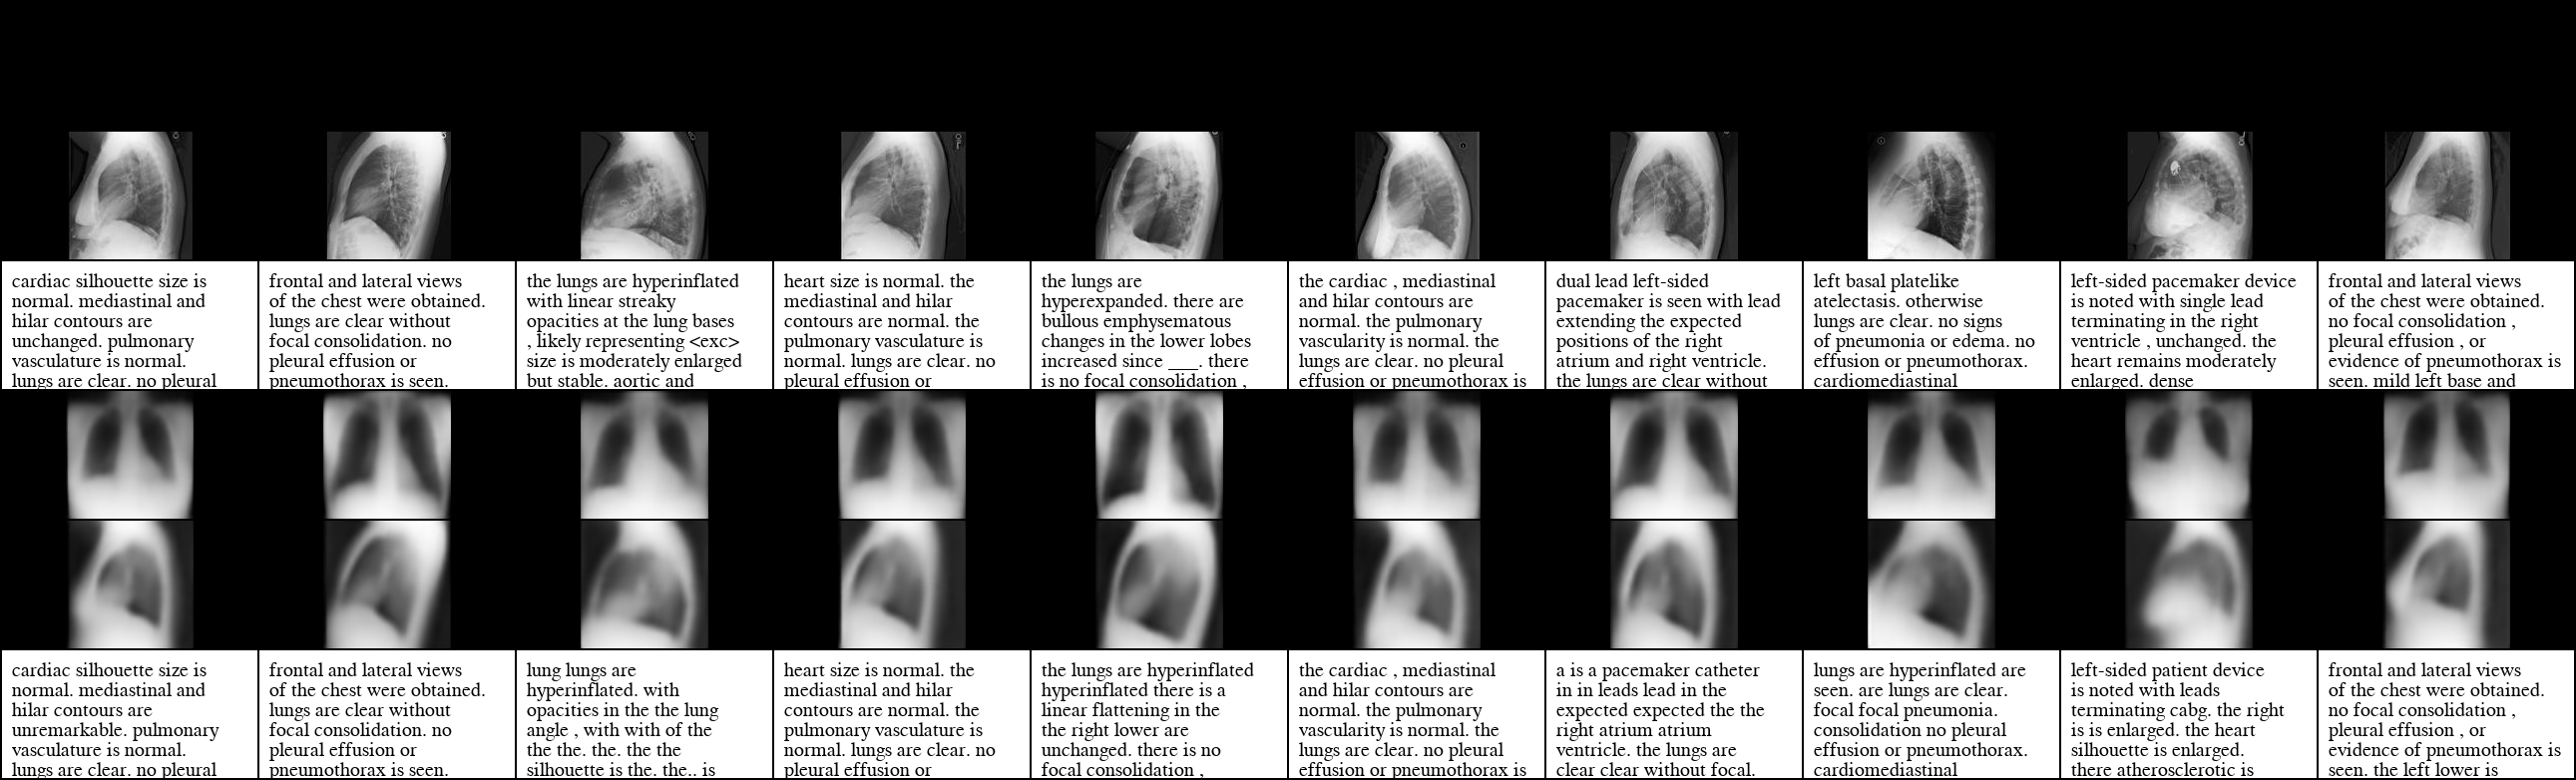
\includegraphics[width=0.6\textwidth, height = \textheight, keepaspectratio]{data/cond_gen/Lateral_text}
                \caption{\tiny{
        \textbf{Conditionally generated samples with F and T modalities as conditioner.} The second and third image rows were given to the model as conditioner. The three last images rows are the generated samples. The images in the first row are the scans that correspond to the samples given as conditioner. The generated samples are blurry and it is difficult to see whether they represent some of the features that are characteristic to the input samples.
    }}
        \end{figure}
    \end{frame}

    \printbibliography
\end{document}
